% !TeX program = xelatex
\documentclass{beamer}
\usepackage{ctex}
\usepackage{hyperref}

\title{Hacking Git - a Blocktree}
\author{陈嘉杰}
\date{2018 年 10 月}

\begin{document}
\begin{frame}
    \maketitle
\end{frame}

\begin{frame}{Git 是个{\bf 啥子}}
    大家知道 Git 是什么吗?
    
    \includegraphics<1->[width=\linewidth]{2018-10-25-08-44-33.png}

    \pause
    the stupid content tracker

    \pause
    a block tree
\end{frame}

\begin{frame}{先开始动手}
    咱们边做边讲,先请大家安装一下 Git :

    \$ apt install -y git

    \pause

    然后设置一下自己的名字和邮箱:

    \$ git config -{}-global user.name "Jiajie Chen"

    \$ git config -{}-global user.email "jiegec@qq.com"

    \pause

    然后新建一个文件夹,在里面建立一个空的 Git 仓库:

    \$ mkdir learn\_git

    \$ cd learn\_git

    \$ git init

\end{frame}

\begin{frame}{Git 能做什么}
    Git 是一个 “版本控制系统” ,这意味着:

    \begin{itemize}
        \item 保存你文件修改的历史记录,你可以看到你以前在什么时候都做了什么更改
        \item 可以多人同时工作在同一个项目里,合理地把大家写的代码合并
        \item 学好了 Git ,有利于软工等课程的学习
        \item 学会了 Git ,你就可以参与到 GitHub 的广阔开发者社区中
        \item 学会了 Git ,你才能有朝一日成为 Linux Kernel 开发者
    \end{itemize}

    不要怕,让我们一点一点来。最后自然也有给大家的一个挑战环节。
\end{frame}

\begin{frame}[fragile]{保存文件历史记录}
    假如要记录和妹子的出游记录(基于 NanoApe 真实事件改编)

    \$ echo "2018-10-04 Shenyang" >{}> log.txt

    \$ git status
    
    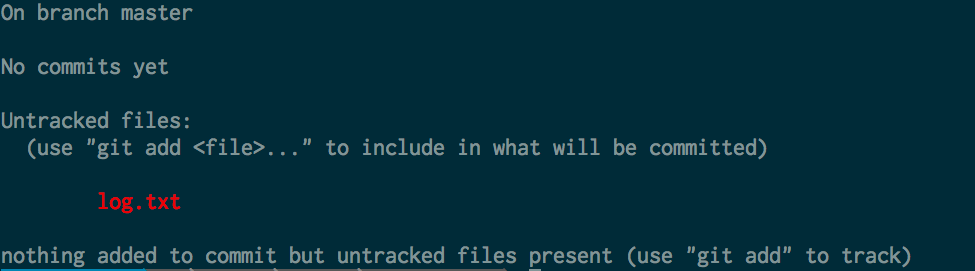
\includegraphics[width=\linewidth]{2018-10-25-09-30-24.png}
\end{frame}

\begin{frame}{git add}
    Git 默认情况下不会把你的文件考虑进来。你必须告诉 Git 让它替你管理这个文件的历史记录。我们采用的命令是:

    \$ git add log.txt

    当然了,它还有别的写法,我们经常会用

    \$ git add .

    来把当前目录和所有子目录里文件都加进来。执行以后,是这个效果:
    
    \$ git status

    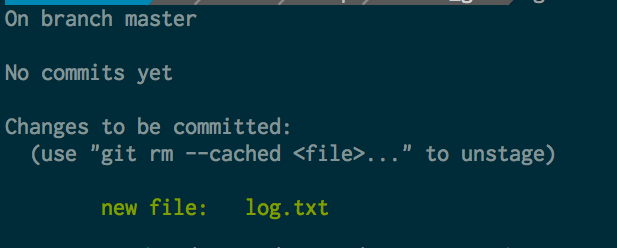
\includegraphics[width=\linewidth]{2018-10-25-09-33-45.png}

\end{frame}

\begin{frame}{年轻人的第一个提交!}
    Git 有暂存区(stage)的概念,允许你在最终决定一个版本前先做一些修改。git add 把当前文件系统的更改添加到暂存区,而 git commit 则把暂存区的更改保存在历史记录中。

    首先我们可以看看暂存区有什么内容:

    \$ git diff --cached
    
    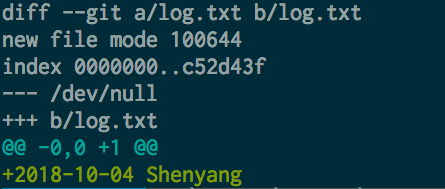
\includegraphics[width=\linewidth]{2018-10-25-09-49-00.png}

    这个格式叫做 Unified Diff 。以后大家还会经常看到。
\end{frame}

\begin{frame}{年轻人的第一个提交!(续)}
    然后 NanoApe 检查了一下,时间和地点都没错,保存!

    \$git commit -m "Add shenyang tour"

    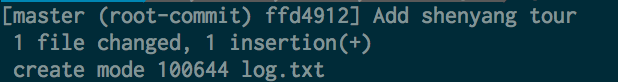
\includegraphics[width=\linewidth]{2018-10-25-09-55-12.png}

    我们再看一下当前的状态:

    \$ git status

    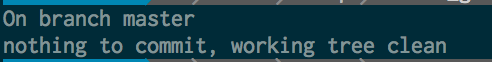
\includegraphics[width=\linewidth]{2018-10-25-09-55-36.png}

    妙啊,我的文件都已经保存进去了。那我想看我之前都做了什么,怎么办?
\end{frame}

\begin{frame}{git log}
    有一个命令可以查看最近的提交: git log

    \$ git log
    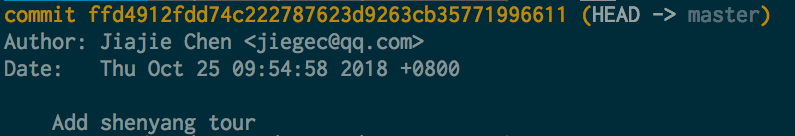
\includegraphics[width=\linewidth]{2018-10-25-09-59-01.png}

    可以看到我在这个时候添加了一个提交,作者是我,时间是这个时间,然后这个提交的描述是这个。

\end{frame}
\begin{frame}{git log (续)}
    怎么看这个提交具体做了什么呢?

    \$ git log -p

    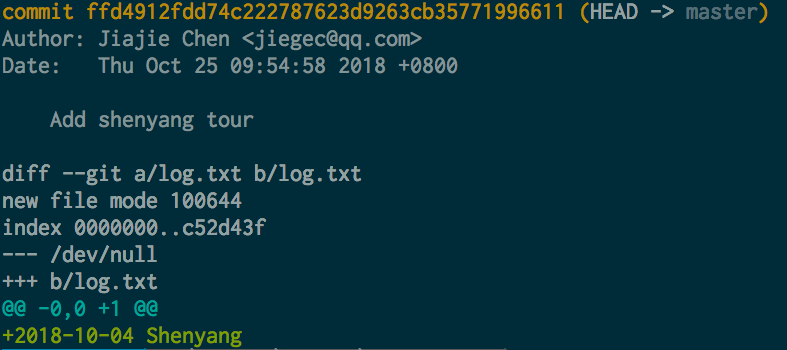
\includegraphics[width=\linewidth]{2018-10-25-10-01-41.png}
\end{frame}

\begin{frame}{一个提交太单调,我们加多一个}
    \$ echo "2018-10-24 128 Days" >{}> log.txt

    \$ git commit -a -m "Add 1024 day"

    \$ git log -p

    注: git commit -a -m "abc" 相当于 git add . \&\& git commit -m "abc"

\end{frame}

\begin{frame}
    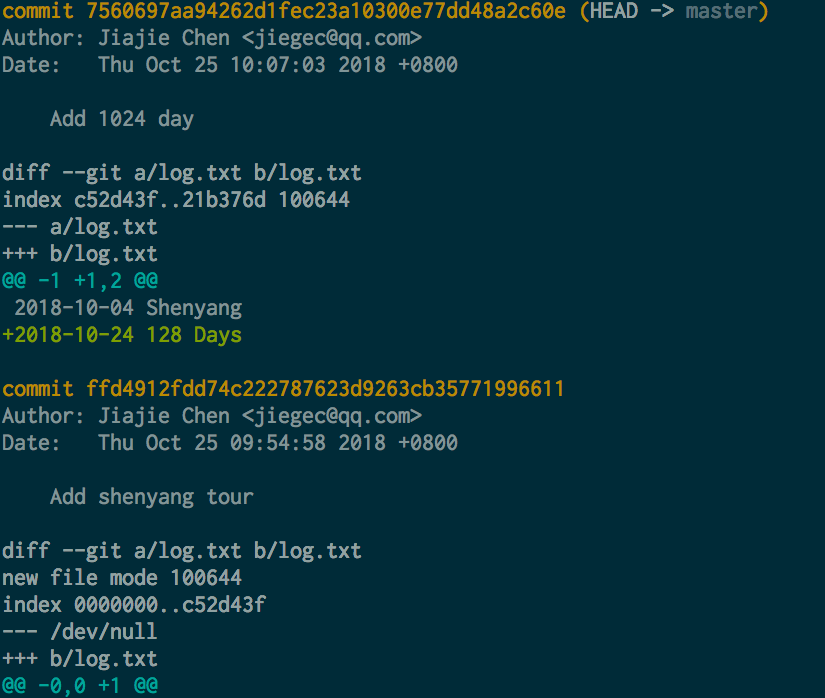
\includegraphics[width=\linewidth]{2018-10-25-10-46-39.png}
\end{frame}

\begin{frame}{啊,忘了一件事情}
    NanoApe: 唔,忘记提妹子的 ID 了,这不行。我得改一下

    \$ cat log.txt

    2018-10-04 Shenyang

    2018-10-24 128 Days with muvseea

    \$ git status

    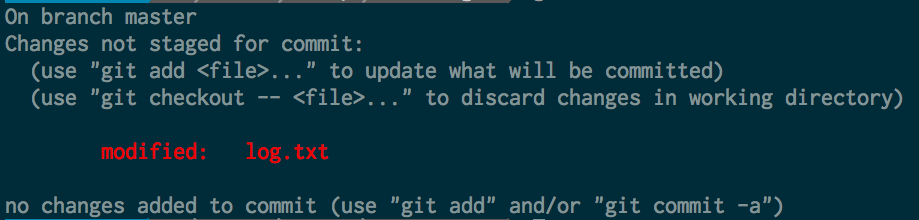
\includegraphics[width=\linewidth]{2018-10-25-10-49-26.png}
\end{frame}

\begin{frame}{啊,忘了一件事情(续)}
    我们可以看到刚刚的更改:

    \$ git diff

    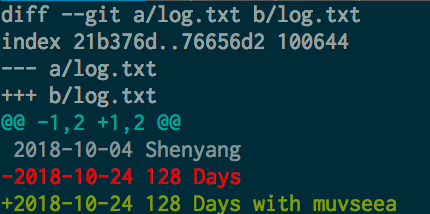
\includegraphics[width=\linewidth]{2018-10-25-10-50-20.png}
\end{frame}

\begin{frame}{啊,忘了一件事情(续续)}
    我看刚才的提交不爽,可不可以更改我上一次的提交?可以:

    \$ git comment -a --amend -m "Add 128 days with muvseea"

    \$ git log

    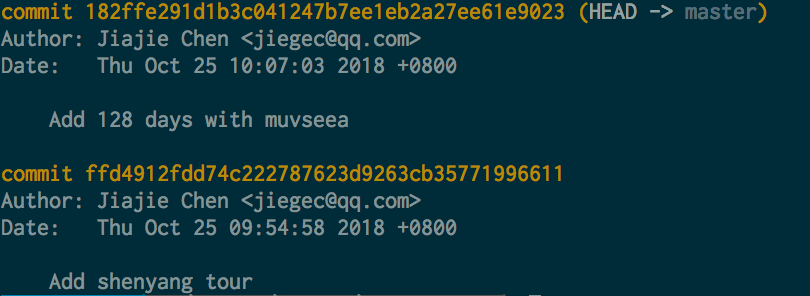
\includegraphics[width=\linewidth]{2018-10-25-10-52-16.png}
\end{frame}

\begin{frame}{谈谈暂存区}
    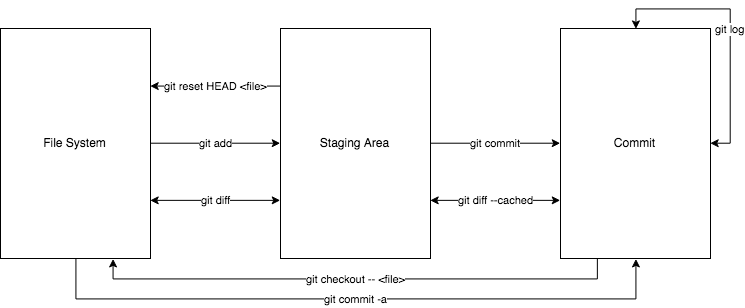
\includegraphics[width=\linewidth]{2018-10-25-11-01-32.png}

    "git status" is your firend.
\end{frame}

\begin{frame}{Pro Git 上的类似表述}
    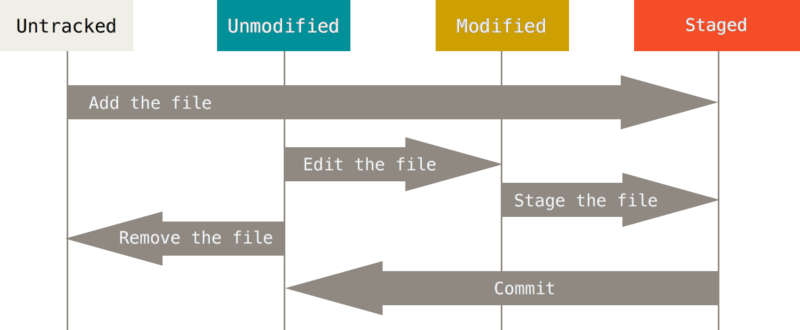
\includegraphics[width=\linewidth]{lifecycle.png}
\end{frame}

\begin{frame}{发布虐狗版本!}
    \$ git tag nue-gou-1.0

    \$ git log

    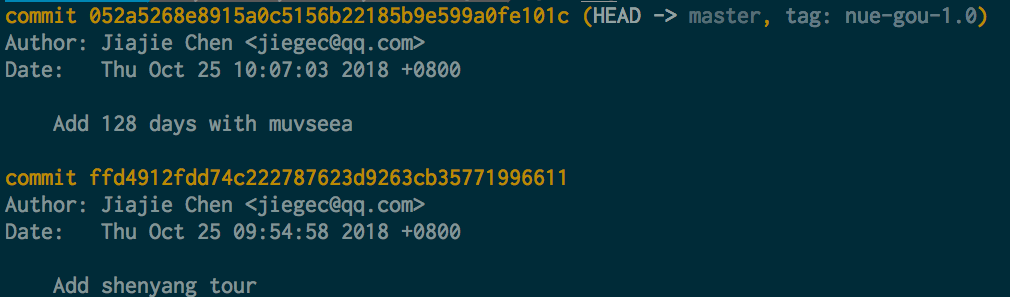
\includegraphics[width=\linewidth]{2018-10-25-11-16-26.png}

    这样我们就创建了一个名为 nue-gou-1.0 的 tag 。查看所有的 tag :

    \$ git tag

    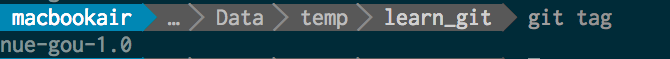
\includegraphics[width=\linewidth]{2018-10-25-11-18-36.png}
\end{frame}

\begin{frame}{虐狗回顾}
    假如 NanoApe 虐狗了 99 年的时候,想看一下当年的自己?(好浪漫啊)

    \$ git checkout -b nue-gou-1.0

    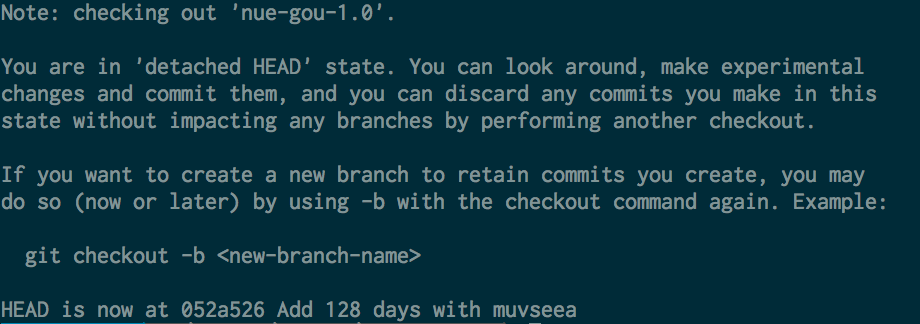
\includegraphics[width=\linewidth]{2018-10-25-11-21-49.png}

    这样就可以回到当时的这个版本。实际上就是对某个 commit 进行了命名。
\end{frame}

\begin{frame}{Git 协作}
    经过上面这部分,你应该已经学会如何用 Git 管理自己的代码了。但 Git 的强大很大程度在于,可以让很多人一起在一个项目上工作。

    我们以清华 Git 为例。

    \url{https://git.tsinghua.edu.cn}

    
\includegraphics[width=\linewidth]{2018-10-25-11-31-40.png}

    使用清华 ID 登录即可。
\end{frame}

\begin{frame}{GitLab 配置}
    进去后,点击右上角的图标,点击 Settings

    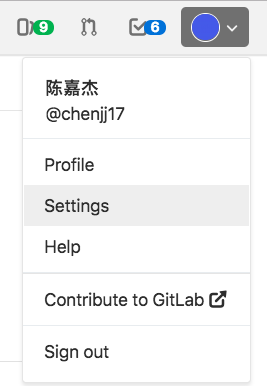
\includegraphics[width=0.5\linewidth]{2018-10-25-11-37-23.png}
\end{frame}

\begin{frame}{GitLab 配置(续)}
    在左下角找到 SSH Keys

    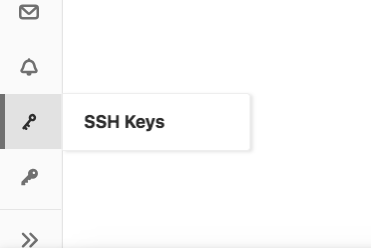
\includegraphics[width=\linewidth]{2018-10-25-11-38-45.png}
\end{frame}

\begin{frame}{GitLab 配置(续续)}
    如果大家还没有生成过,回到终端,生成一个自己的 SSH Key :

    \$ ssh-keygen

    按照要求生成 SSH Key 。注意保存!拥有这个 Key 就可以对你拥有的 GitLab 仓库进行修改。

    然后查看 \~{}/.ssh/id\_rsa.pub 文件的内容,复制到浏览器中,输入一个名称,最后添加到 GitLab 中。效果如图:

    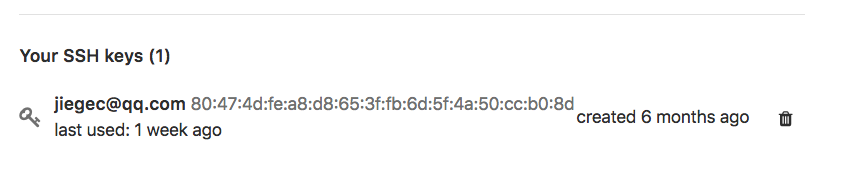
\includegraphics[width=\linewidth]{2018-10-25-11-42-06.png}

    测试一下是否成功配置了:

    \$ ssh -T git@git.tsinghua.edu.cn

    应该会输出 Welcome To GitLab 的信息。

\end{frame}

\begin{frame}{创建仓库}
    找到 New Project ,进入创建仓库界面 \url{https://git.tsinghua.edu.cn/projects/new}

    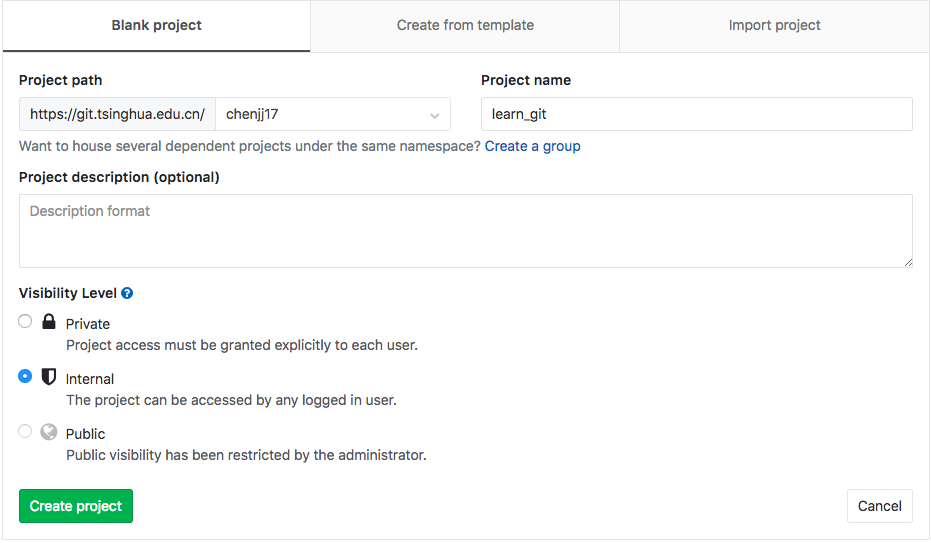
\includegraphics[width=\linewidth]{2018-10-25-11-54-08.png}

    点击 Create Project 。

\end{frame}

\begin{frame}{把刚才的仓库推到 GitLab 上}
    \$ git remote add origin git@git.tsinghua.edu.cn:chenjj17/learn\_git.git
    
    \$ git push origin master

    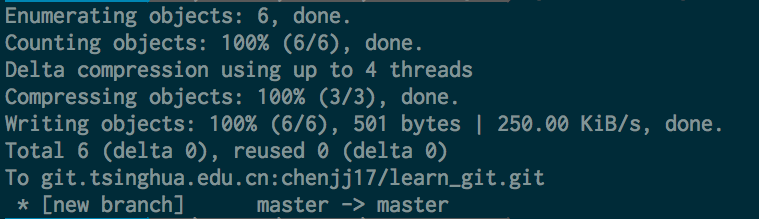
\includegraphics[width=\linewidth]{2018-10-25-11-59-01.png}
\end{frame}
\end{document}
